%%%%%%%%%%%%%%%%%%%%%%%%%%%%%%%%%%%%%%%%%%%%%%%%
% E.Pinault-Bigeard - e.pinault-bigeard@upsti.fr
% http://s2i.pinault-bigeard.com
% CC BY-NC-SA 2.0 FR - http://creativecommons.org/licenses/by-nc-sa/2.0/fr/
%%%%%%%%%%%%%%%%%%%%%%%%%%%%%%%%%%%%%%%%%%%%%%%%
\documentclass[11pt]{article}
%%%%%%%%%%%%%%%%%%%%%%%%%%%%%%%%%%%%%%%%%%%%%%%%
% Package UPSTI_Document
%%%%%%%%%%%%%%%%%%%%%%%%%%%%%%%%%%%%%%%%%%%%%%%%
%%%%%%%%%%%%%%%%%%%%%%%%%%%%%%%%%%%%%%%%%%%%%%%%
% Package UPSTI_Document
%%%%%%%%%%%%%%%%%%%%%%%%%%%%%%%%%%%%%%%%%%%%%%%%
\usepackage{subcaption}
\usepackage[usenames, svgnames, dvipsnames]{xcolor}
\usepackage{UPSTI_Document}
\usepackage{pgfplots}
\usepackage{import}
\definecolor{darkspringgreen}{rgb}{0.09, 0.45, 0.27}

\newcommandx*{\dessinRepereFigGeo}[5][1=\vx{},2=\vy{},3=\vz{},4=,5=0]
	{
		\draw [->,very thick] (0,0) -- (1,0) ;
		\draw [->,very thick] (0,0) -- (0,1) ;
    \fill[white] (0,0) circle (0.13);
    \draw [->,very thick] (0,0) circle (0.13);
    \ifnumequal{#5}{0} {% z vers nous
      \fill[black] (0,0) circle (0.03);
      \draw [->,thick] (0,0) circle (0.04);
    }{% z vers la feuille
  		\begin{scope} [rotate=45]
  			\draw [-,thick] (0,-0.12) -- (0,0.12) ;
  			\draw [-,thick] (-0.12,0) -- (0.12,0) ;
  		\end{scope}
    }
		\draw [anchor=north west] (1.1,0) node {${#1}$};
		\draw [anchor=south west] (0,1.1) node {${#2}$};
		\draw [anchor=north east] (-0.1,0) node {${#3}$};
		\draw [anchor=north west] (-0.1,-0.1) node {${#4}$};
	}

	\usepackage{array}
	\newcolumntype{L}[1]{>{\raggedright\let\newline\\\arraybackslash\hspace{0pt}}m{#1}}
	\newcolumntype{C}[1]{>{\centering\let\newline\\\arraybackslash\hspace{0pt}}m{#1}}
	\newcolumntype{R}[1]{>{\raggedleft\let\newline\\\arraybackslash\hspace{0pt}}m{#1}}

	\usepackage{pifont}% http://ctan.org/pkg/pifont
\newcommand{\cmark}{\color{green}\ding{51}}%
\newcommand{\xmark}{\color{red}\ding{55}}%
\newcommand{\fmark}{\ding{229}}%
\newcommand{\itemc}{\item[\cmark]}%
\newcommand{\itemx}{\item[\xmark]}%
\newcommand{\itemf}{\item[\fmark]}%


%---------------------------------%
% Paramètres du package
%---------------------------------%

% Version du document (pour la compilation)
% 1: Document prof
% 2: Document élève
% 3: Document à publier
\newcommand{\UPSTIidVersionDocument}{2}


% Variante
%\newcommand{\UPSTIvariante}{2}

% Classe
% 1: PTSI				6: PSI*			11: TSI2		16: Spé
% 2: PT	(par défaut)	7: MPSI			12: ATS
% 3: PT*				8: MP			13: PC
% 4: PCSI				9: MP*			14: PC*
% 5: PSI				10: TSI1		15: Sup
%\newcommand{\UPSTIidClasse}{2}



% Matière
% 1: S2I (par défaut)    2: IPT     3: TIPE
% 6: Vie au lycée
\newcommand{\UPSTIvariante}{5}
\newcommand{\UPSTIidMatiere}{0}
\newcommand{\UPSTIintituleMatiere}{Automatique}
\newcommand{\UPSTIsigleMatiere}{Autom}
% Type de document
% 0: Custom*				7: Fiche Métho de			14: Document Réponses
% 1: Cours (par défaut)		8: Fiche Synthèse    		15: Programme de colle
% 2: TD     				9: Formulaire
% 3: TP						10: Memo
% 4: Colle					11: Dossier Technique
% 5: DS						12: Dossier Ressource
% 6: DM						13: Concours Blanc
% * Si on met la valeur 0, il faut décommenter la ligne suivante:
%\newcommand{\UPSTItypeDocument}{Custom}
\newcommand{\UPSTIidTypeDocument}{1}

% Titre dans l'en-tête


% Titre dans l'en-tête

\newcommand{\UPSTIvariante}{5}

\newcommand{\UPSTItitreEnTete}{Automatisme industriel}
%\newcommand{\UPSTItitreEnTetePages}{}
\newcommand{\UPSTIsousTitreEnTete}{Introduction aux API}


% Titre
%\newcommand{\UPSTItitrePreambule}{Automatisme industriel}
\newcommand{\UPSTItitre}{La programmation d'un Automate Industriel}

% Durée de l'activité (pour DS, DM et TP)
\newcommand{\UPSTIduree}{3h30}

% Note de bas de première page
%\newcommand{\UPSTInoteBasDePremierePage}{Geoffrey Vaquette}
% Numéro (ajoute " n°1" après DS ou DM)
\newcommand{\UPSTInumero}{2}

% Numéro chapitre
%\newcommand{\UPSTInumeroChapitre}{1}

% En-tête customisé
%\newcommand{\UPSTIenTetePrincipalCustom}{UPSTIenTetePrincipalCustom}

% Message sous le titre
%\newcommand{\UPSTImessage}{Message sous le titre}


% Référence au programme
%\newcommand{\UPSTIprogramme}{\EPBComp \EPBCompP{B1-02}, \EPBCompP{B2-49}, \EPBCompS{B2-50}, \EPBCompS{B2-51}, \EPBCompP{C1-07}, \EPBCompP{C1-08}}

% Si l'auteur n'est pas l'auteur par défaut
%\renewcommand{\UPSTIauteur}{WWOOOOOOWW}

% Si le document est réalisé au nom de l'équipe
%\newcommand{\UPSTIdocumentCollegial}{1}

% Source
%\newcommand{\UPSTIsource}{UPSTI}

% Version du document
\newcommand{\UPSTInumeroVersion}{0.1}

%-----------------------------------------------
\UPSTIcompileVars		% "Compile" les variables
%%%%%%%%%%%%%%%%%%%%%%%%%%%%%%%%%%%%%%%%%%%%%%%%

\include{dirtree}
%%%%%%%%%%%%%%%%%%%%%%%%%%%%%%%%%%%%%%%%%%%%%%%%
% Début du document
%%%%%%%%%%%%%%%%%%%%%%%%%%%%%%%%%%%%%%%%%%%%%%%%
\usepackage{grafcet}

\usetikzlibrary[circuits.plc.ladder]            %     
\newlength{\ladderskip}\setlength{\ladderskip}{5\tikzcircuitssizeunit}%5\tikzcircuitssizeunit    = 355pt
\newlength{\ladderrungsep}
\setlength{\ladderrungsep}{.2\ladderskip}
\def\ladderrungend#1{\pgftransformyshift{-#1\ladderskip-\ladderrungsep}}


\begin{document}
\UPSTIbuildPage

\tableofcontents

\section*{Introduction}
Le logiciel de développement d'un API (Automate Programmable Industriel) est un logiciel permettant de configurer et de programmer l'API associé. Chaque constructeur d'API  impose son propre logiciel de développement.

\begin{table}[ht]
\centering
	\begin{tabular}{c|c|c|c}
 \textbf{Schneider} & \textbf{Siemens} & \textbf{Wago} & \textbf{Tend} \\\hline
 Unity Pro & Tia Portal & CodeSys & Niagara \\
 EcoStructure & & eCockpit & \\
\end{tabular}

	\caption{Logiciel de développement pour chaque constructeur.}
\end{table}


Le langage LADDER fut conçu dans les années 1970 pour faire passer les électrotechniciens de la saisie de schémas électriques de systèmes à relais  à la programmation.
Il est donc simple et proche de la description de schémas électriques.
On le réserve à la description de fonctions combinatoires ou à des calculs simples.

Une ligne d'un programme LADDER est appelée réseau.

Un réseau est composé de contacts, de bobine et/ou de blocs.

\subsection{Réseaux LADDER simples}

\subsubsection{Les contacts}

Les contacts représentent des entrées logiques (TOR).

\UPSTIaRetenir{Il existe deux types de contacts :
\begin{description}
  \item [$\begin{array}{l}\begin{tikzpicture}[circuit plc ladder,thick,x=\ladderskip,y=\ladderskip]
  \draw(0,0) to [contact NO={info={a}}] ++ (1,0);
\end{tikzpicture}
 \end{array}$] \textbf{Contact normalement ouvert} :
  actif lorsque la variable associée est à l'état 1.
  \begin{itemize}
    \item [$\Rightarrow$] Il représente donc la variable $a$
  \end{itemize}
  \item [$\begin{array}{l}\begin{tikzpicture}[circuit plc ladder,thick,x=\ladderskip,y=\ladderskip]
  \draw(0,0) to [contact NC={info={a}}] ++ (1,0);
\end{tikzpicture}
 \end{array}$]  \textbf{Contact normalement fermé } actif lorsque la variable associée est à l'état 0.
  \begin{itemize}
    \item [$\Rightarrow$] Il représente donc la variable $\overline{a}$
  \end{itemize}
\end{description}
}

\subsubsection{Les bobines}

Les bobines représentent les sorties logiques (TOR) de l'API.

\UPSTIaRetenir{Une sortie S de l'automate est active lorsque la bobine associée $\begin{array}{l}\begin{tikzpicture}[circuit plc ladder,thick,x=\ladderskip,y=\ladderskip]
  \draw(0,0) to [coil={info={S}}] ++ (1,0);
\end{tikzpicture}
\end{array}$ est active.}


\subsubsection{Réseaux de base}

La traduction en réseau LADDER de l'équation $S = a$ est donc représentée sur la figure \ref{fig:ladAtoS}. L'équation en réseau LADDER de l'équation $S = \overline{a}$ est représentée sur la figure~\ref{fig:ladABartoS}

\begin{figure}[ht]
  \begin{subfigure}[b]{.49\textwidth}
  \centering
    \begin{tikzpicture}[circuit plc ladder, thick, x=\ladderskip, y=\ladderskip]
  \draw(0,0) to [contact NO={info={a}}] ++ (1,0) -- ++(1,0)
    to [coil={info={Sortie}}] + (1,0) coordinate(laddertopright);
    \ladderrungend{1.2}
    \draw let \p1=(laddertopright) in
    (0,   \y1+0.7\ladderskip) -- (0,    \ladderskip)
    (\x1, \y1+0.7\ladderskip) -- (\x1,  \ladderskip);
\end{tikzpicture}

    \caption{$S = a$}
    \label{fig:ladAtoS}
  \end{subfigure}
  %
  \begin{subfigure}[b]{.49\textwidth}
  \centering
    \begin{tikzpicture}[circuit plc ladder, thick, x=\ladderskip, y=\ladderskip]
  \draw(0,0) to [contact NC={info={a}}] ++ (1,0) -- ++(1,0)
    to [coil={info={Sortie}}] + (1,0) coordinate(laddertopright);
    \ladderrungend{1.2}
    \draw let \p1=(laddertopright) in
    (0,   \y1+0.7\ladderskip) -- (0,    \ladderskip)
    (\x1, \y1+0.7\ladderskip) -- (\x1,  \ladderskip);
\end{tikzpicture}

    \caption{$S = \overline{a}$}
    \label{fig:ladABartoS}
  \end{subfigure}

  \caption{Réseaux LADDER de base}
\end{figure}

Comme dans un circuit électrique, il est possible de programmer des équation combinatoires en langage LADDER. Les fonctions \textbf{ET} et \textbf{OU} sont représentée sur la figure~\ref{fig:equaLogiques}

\begin{figure}[ht]
  \begin{subfigure}[b]{.49\textwidth}
    \centering
    \begin{tikzpicture}[circuit plc ladder, thick, x=\ladderskip, y=\ladderskip]
  \draw(0,0) to [contact NO={info={a}}] ++ (1,0)
    to [contact NO={info={b}}] ++ (1,0) -- ++(1,0)
    to [coil={info={Sortie}}] + (1,0) coordinate(laddertopright);
    \ladderrungend{1.2}
    \draw let \p1=(laddertopright) in
    (0,   \y1+0.7\ladderskip) -- (0,    \ladderskip)
    (\x1, \y1+0.7\ladderskip) -- (\x1,  \ladderskip);
\end{tikzpicture}

    \caption{$S = a \text{ ET } b$}
    \label{fig:aETb}
  \end{subfigure}
  %
  \begin{subfigure}[b]{.49\textwidth}
    \centering 
    \begin{tikzpicture}[circuit plc ladder,thick,x=\ladderskip,y=\ladderskip]
  \draw(0,0) to [contact NO={info={a}}] ++ (1,0) coordinate(laddercoil) -- ++(2,0) to [coil={info={Sortie}}] ++ (1,0) coordinate(laddertopright);
  \draw(0,-1) to [contact NO={info={b}}] ++ (1,0) -- (laddercoil);

  \ladderrungend{2}
  \draw let \p1=(laddertopright) in
  (0,   \y1+0.7\ladderskip) -- (0,    \ladderskip)
  (\x1, \y1+0.7\ladderskip) -- (\x1,  \ladderskip);
\end{tikzpicture}

    \caption{$S = a \text{ OU } b$}
    \label{fig:aOUb}
  \end{subfigure}
  \caption{Equations logiques simples}
  \label{fig:equaLogiques}
\end{figure}

\begin{UPSTIactivite}
    \UPSTIquestion{Dessinez le réseau LADDER de l'équation $S = a + \overline{b}$}

    \UPSTIlignesACompleter[2]{\begin{center}
      \input{ladder_diagrams/ladCircuitaOubBar.tikz}
    \end{center}}

    \UPSTIquestion{Dessinez le réseau LADDER de l'équation $S = \overline{a} \cdot \overline{b}$}

    \UPSTIlignesACompleter[2]{\begin{center}
      \begin{tikzpicture}[circuit plc ladder, thick, x=\ladderskip, y=\ladderskip]
  \draw(0,0) to [contact NC={info={a}}] ++ (1,0)
    to [contact NC={info={b}}] ++ (1,0) -- ++(1,0)
    to [coil={info={Sortie}}] + (1,0) coordinate(laddertopright);
    \ladderrungend{2}
    \draw let \p1=(laddertopright) in
    (0,   \y1+0.7\ladderskip) -- (0,    \ladderskip)
    (\x1, \y1+0.7\ladderskip) -- (\x1,  \ladderskip);
\end{tikzpicture}

    \end{center}}

    \UPSTIquestion{Dessinez le réseau LADDER de l'équation $S = (a + b) \cdot \overline{b} \cdot c $}

    \UPSTIlignesACompleter[2]{\begin{center}
      \begin{tikzpicture}[circuit plc ladder,thick,x=\ladderskip,y=\ladderskip]
  \draw(0,0) to [contact NO={info={a}}] ++ (1,0) coordinate(laddercoil)
  to [contact NC={info={b}}] ++ (1,0) 
  to [contact NO={info={c}}] ++ (1,0)
  -- ++(2,0) to [coil={info={Sortie}}] ++ (1,0) coordinate(laddertopright);
  \draw(0,-1) to [contact NO={info={b}}] ++ (1,0) -- (laddercoil);

  \ladderrungend{2}
  \draw let \p1=(laddertopright) in
  (0,   \y1+0.7\ladderskip) -- (0,    \ladderskip)
  (\x1, \y1+0.7\ladderskip) -- (\x1,  \ladderskip);
\end{tikzpicture}

    \end{center}}


\end{UPSTIactivite}


\section{Le langage GRAFCET}

Le langage GRAFCET, aussi appelé SFC (Sequentiel Function Chart) est, comme son nom l'indique, dédié à la description et à la programmation de \textbf{problèmes séquentiels}. Il décrit donc une suite d'étapes séparées par des transitions.

Un GRAFCET est très proche conceptuellement d'une machine à état. Il est représenté tel que sur la Figure~\ref{fig:simpleGrafcet}

\begin{figure}[ht]
  \centering
  \begin{tikzpicture}
\EtapeInit[0,0]{100}
\Transition[VX100]{100}
\Etape[VT100]{110}
\Transition{110}
\Etape[VT110]{120}
\Transition[VX120]{120}
\LienRetour{T120}{X100}
\Recept{T100}{$dcy \cdot a_0$}
\ActionX{X110}{Sortir Noyau}
\Recept{T110}{condition}\ActionX{X120}{Rentrer Noyau}
\Recept{T120}{$a_0$}
\end{tikzpicture}

  \caption{GRAFCET simple composé de trois étapes}
  \label{fig:simpleGrafcet}
\end{figure}

\subsection{Étapes et actions}

Une étape est représentée par un carré comportant un numéro (Figure~\ref{fig:etape}). Elle est généralement associée à une  (Figure~\ref{fig:etapeAction}) ou plusieurs (Figure~\ref{fig:etapeDeuxActions}) actions.
Il est également possible d'ajouter une condition à une action (Figure~\ref{fig:etapeActionCond}).

\UPSTIaRetenir{\begin{itemize}
  \item Une action associée à une étape n'est effectuée que lorsque l'action associée est active.
  \item Une action conditionnelle est effectuée lorsque l'action est active et que la condition associée est vérifiée.
\end{itemize}}

Il également possible d'effectuer une action qu'au moment de l'activation d'une étape (Figure~\ref{fig:etapeActivation}). Cela est particulièrement utile pour incrémenter un compteur.
En effet, sans cela l'action \textit{compteur = compteur + 1} serait effectuée durant toute la durée de l'action associée. Cela incrémenterait le compteur à chaque cycle automate donc toutes les \SI{10}{ms} approximativement.

On peut représenter l'étape actuellement active dans un grafcet à l'aide d'une étoile comme illustré sur la Figure~\ref{fig:etapeActive}.

\begin{figure}[ht]
\centering
  \begin{subfigure}[b]{.49\textwidth}
    \centering
    \begin{tikzpicture}
      \Etape[0,0]{110}
    \end{tikzpicture}
    \caption{Représentation d'une étape en GRAFCET}
    \label{fig:etape}
  \end{subfigure}%
  %
  \begin{subfigure}[b]{.49\textwidth}
    \centering
  \begin{tikzpicture}
    \Etape[0,0]{110}
    \ActionX{X110}{Sortir Noyau}
  \end{tikzpicture}
  \caption{Une étape et l'action associée}
  \label{fig:etapeAction}
  \end{subfigure}%
  %

  \begin{subfigure}[b]{.48\textwidth}
    \centering
  \begin{tikzpicture}
    \Etape[0,0]{110}
    \ActionX{X110}{Sortir Noyau, Allumer voyant}
  \end{tikzpicture}
  \caption{Une étape et deux actions simultanées. Les deux actions sont actives tant que l'étape 110 est active.}
  \label{fig:etapeDeuxActions}
  \end{subfigure}\hfill
%
  \begin{subfigure}[b]{.48\textwidth}
    \centering
  \begin{tikzpicture}
    \Etape[0,0]{110}
    \ActionX{X110}{Sortir Noyau}
    \ActionCond{X110}{$\overline{\text{defaut}}$}
  \end{tikzpicture}
  \caption{Une étape avec action conditionnelle : L'action \textit{Sortir Noyau} ne sera exécutée que si \textit{defaut} est à 0.}
  \label{fig:etapeActionCond}
  \end{subfigure}%

  \begin{subfigure}[b]{.48\textwidth}
    \centering
  \begin{tikzpicture}
    \Etape[0,0]{130}
    \ActionX{X130}{compteur = compteur + 1;}
    \ActionActiv{X130}
  \end{tikzpicture}
  \caption{Une étape et une action sur activation. L'action n'est effectuée qu'au moment de l'activation de l'étape.}
  \label{fig:etapeActivation}
  \end{subfigure}%
  %
  \begin{subfigure}[b]{.48\textwidth}
    \centering
  \begin{tikzpicture}
    \Etape[0,0]{110}
    \ActionX{X110}{Sortir Noyau}
    %\ActionCond{X110}{$\overline{\text{defaut}}$}
    \LienActivation{X110}
  \end{tikzpicture}
  \caption{Etape courramment active}
  \label{fig:etapeActive}
  \end{subfigure}
  \caption{Etapes et action(s) associée(s)}%
  %
\end{figure}


\subsection{Transitions}

Une transition est \textbf{toujours} placée entre deux actions. Ce sont les transitions qui décrivent la façon de passer d'une action à une autre.
Une transition est associée à une \textbf{réceptivité}.

\UPSTIaRetenir{Une transition sera franchie si et seulement si l'étape précédente est active ET la réceptivité associée est vérifiée.}


%\section{Projet Unity Pro}

La Figure~\ref{fig:unity_fenetre} est une capture d'écran d'une fenêtre \textit{Unity Pro}. Sur la gauche se trouve l'Arborescence du projet, décrite dans la section suivante et la grande partie à droite est la partie programmation.

\begin{figure}[hbt]
	\centering
	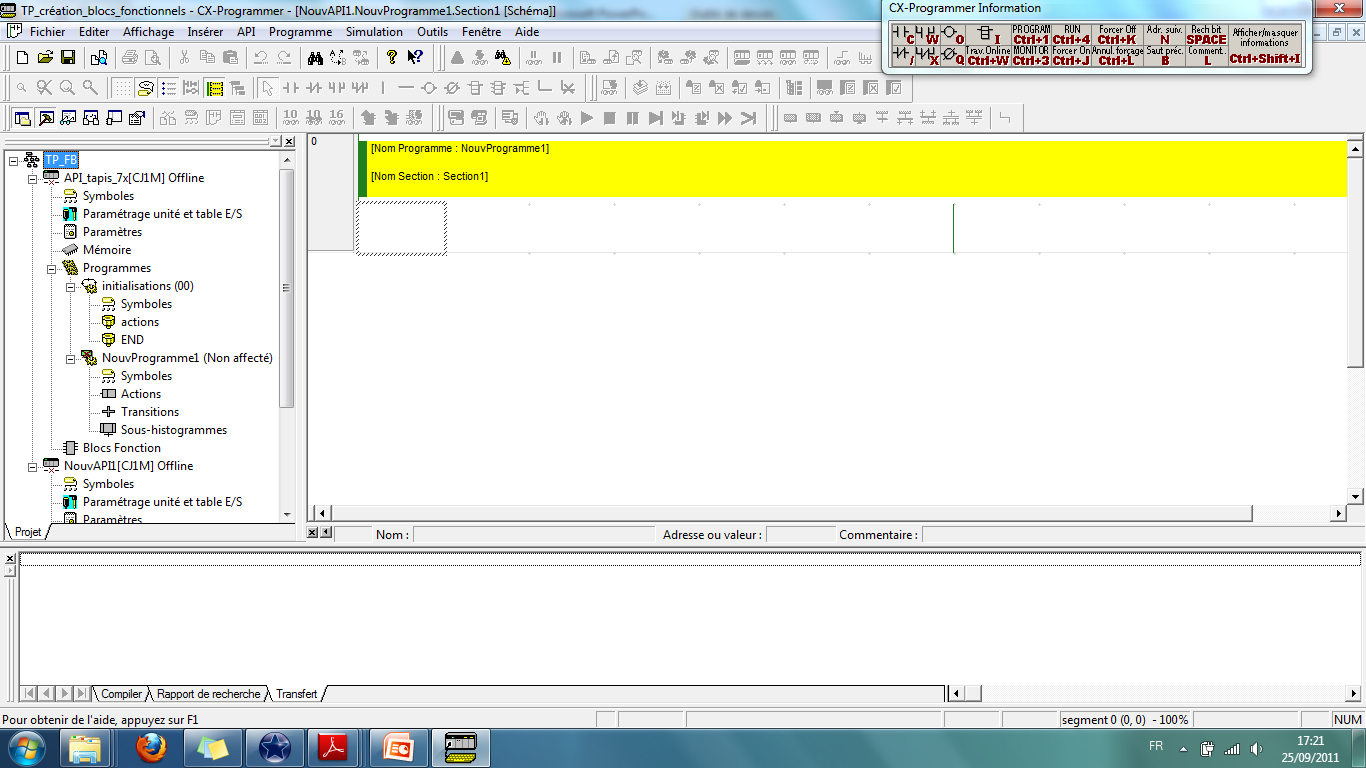
\includegraphics[trim = 0mm 15mm 0mm 0mm, clip,width=.7\linewidth]{images/unity_arbo}
	\caption{Fenêtre Unity Pro}
	\label{fig:unity_fenetre}
\end{figure}

\subsection{L'Arborescence d'un projet Unity}

\begin{figure}[ht]
\centering
\begin{minipage}{.33\linewidth}
	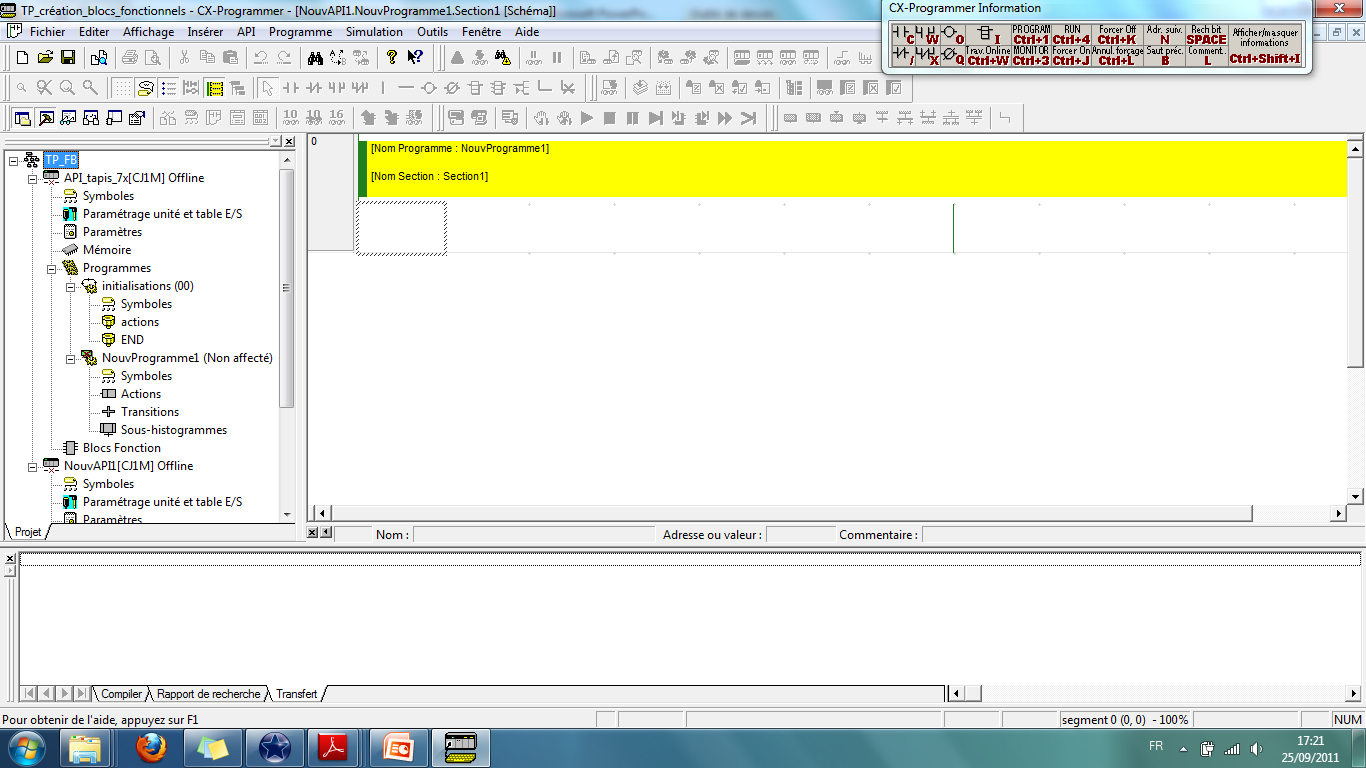
\includegraphics[trim = 2mm 90mm 385mm 53mm, clip, width=\textwidth]{images/unity_arbo}
\end{minipage}\hfill
\begin{minipage}{.63\linewidth}
\dirtree{%
.0 Projet.
.1 API\_Tapis[\dots]/ \DTcomment{Une première configuration}.
	 .2 Symboles \DTcomment{Variables globales}.
	 .2 Paramétrage unité et table E/S.
	 .2 Paramètres \DTcomment{Paramètres de l'automate}.
	 .2 Programmes/ \DTcomment{Programmes dans l'API}.
				.3 Programme\_1/ \DTcomment{Exemple 1 : LADDER}.
					.4 Symboles \DTcomment{Variables locales au programme}.
					.4 actions \DTcomment{Le programme en tant que tel}.
					.4 END.
				.3 Programme\_2/ \DTcomment{Exemple 2 : SFC}.
					.4 Symboles.
					.4 Actions.
					.4 Transitions.
					.4 Sous-histogrammes.
.1 NouvAPI[\dots]/ \DTcomment{Une autre configuration}.
}
\end{minipage}
	\caption{Arborescence d'un projet Unity}
	\label{fig:unity_arbo}
\end{figure}

La Figure~\ref{fig:unity_arbo} présente l'arborescence générale d'un projet \textit{Unity Pro}.

Un projet est constitué de différentes \textbf{configurations} (une configuration pour chaque automate relié au projet). Dans l'exemple de la Figure~\ref{fig:unity_arbo}, les configurations sont 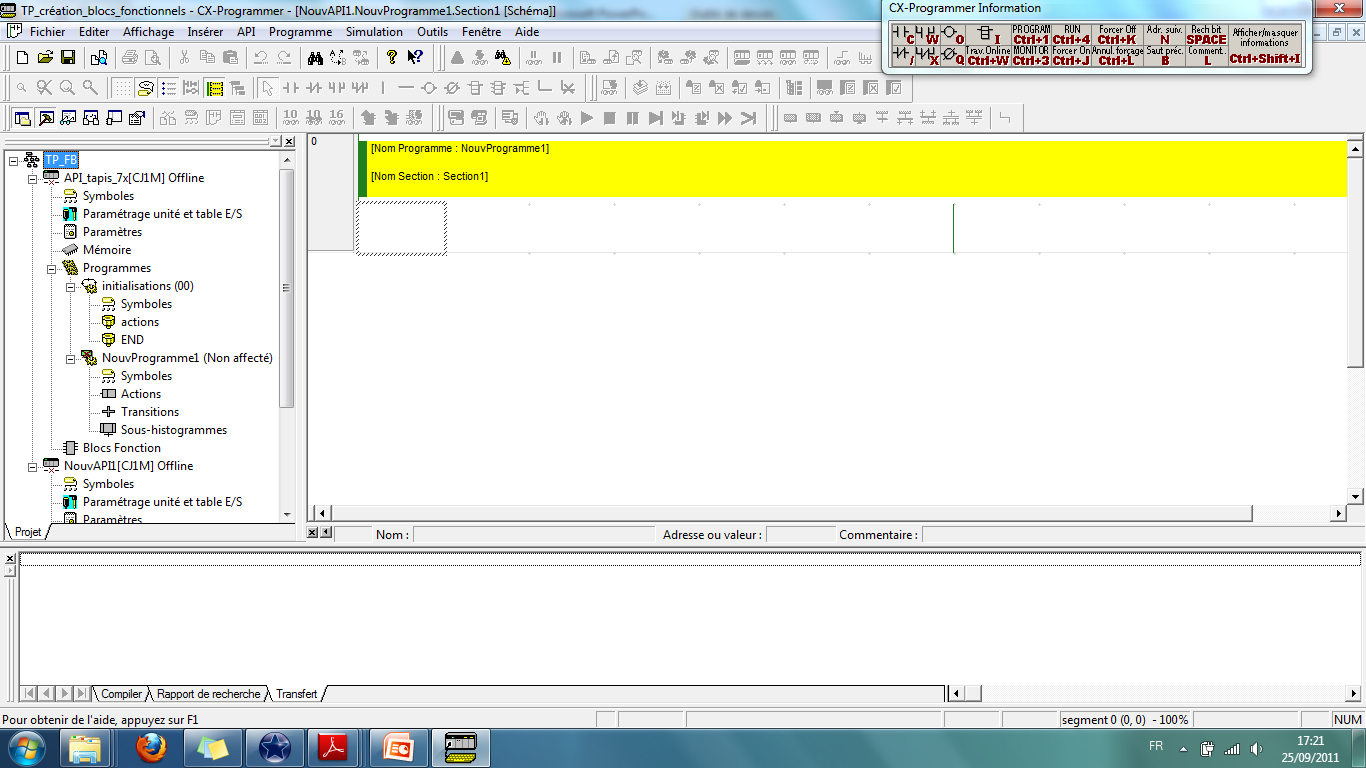
\includegraphics[trim = 40 582 1200 170, clip,height=\fontcharht\font`\B]{images/unity_arbo} et 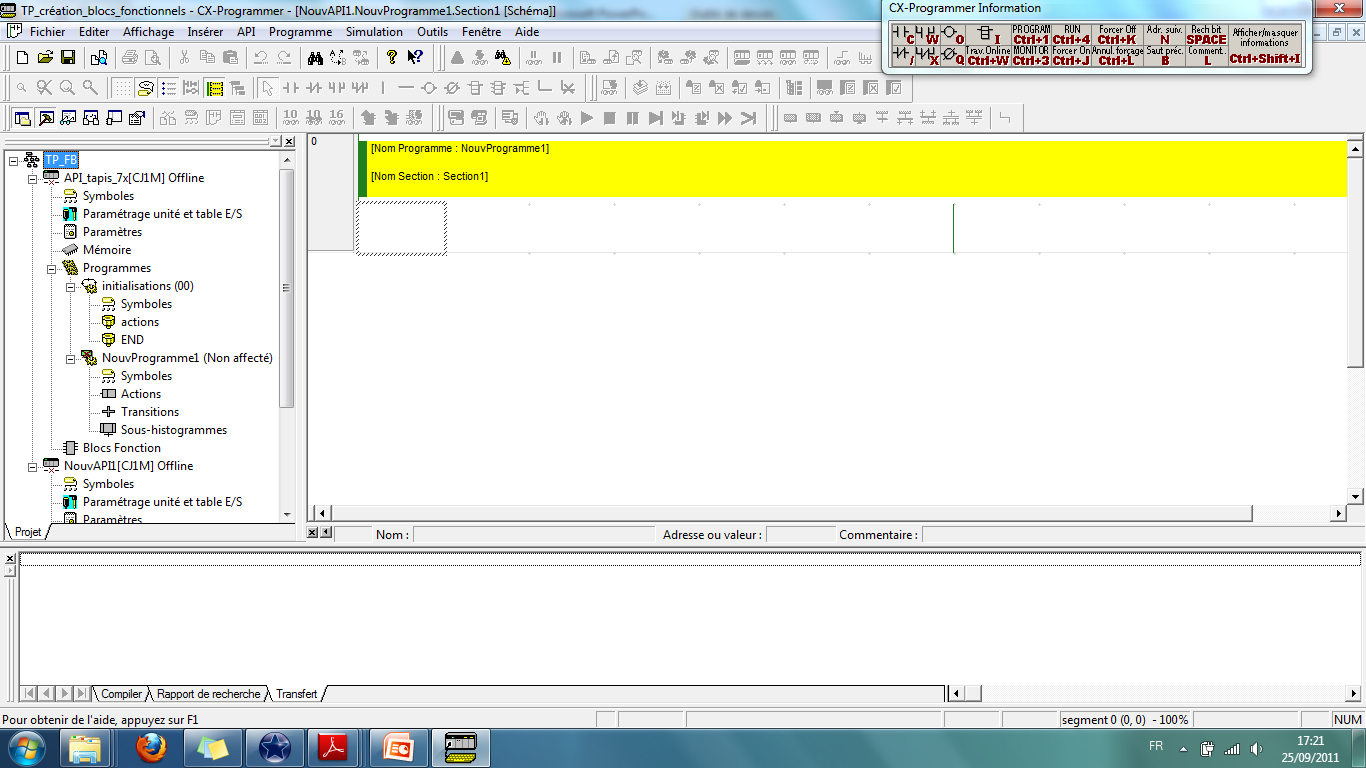
\includegraphics[trim = 40 296 1210 457, clip,height=\fontcharht\font`\B]{images/unity_arbo}.

Dans chaque configuration, on trouve :
\begin{itemize}
	\item Les ressources
		\begin{itemize}
			\item \begin{minipage}[c]{.55\textwidth}
			 	On y trouve la configuration de l'automate, les variables globales (symboles), les déclarations des modules d'entrée-sortie, les registres (mémoire de l'automate) \dots
			\end{minipage}\hfill
			\begin{minipage}[c]{.3\textwidth}
				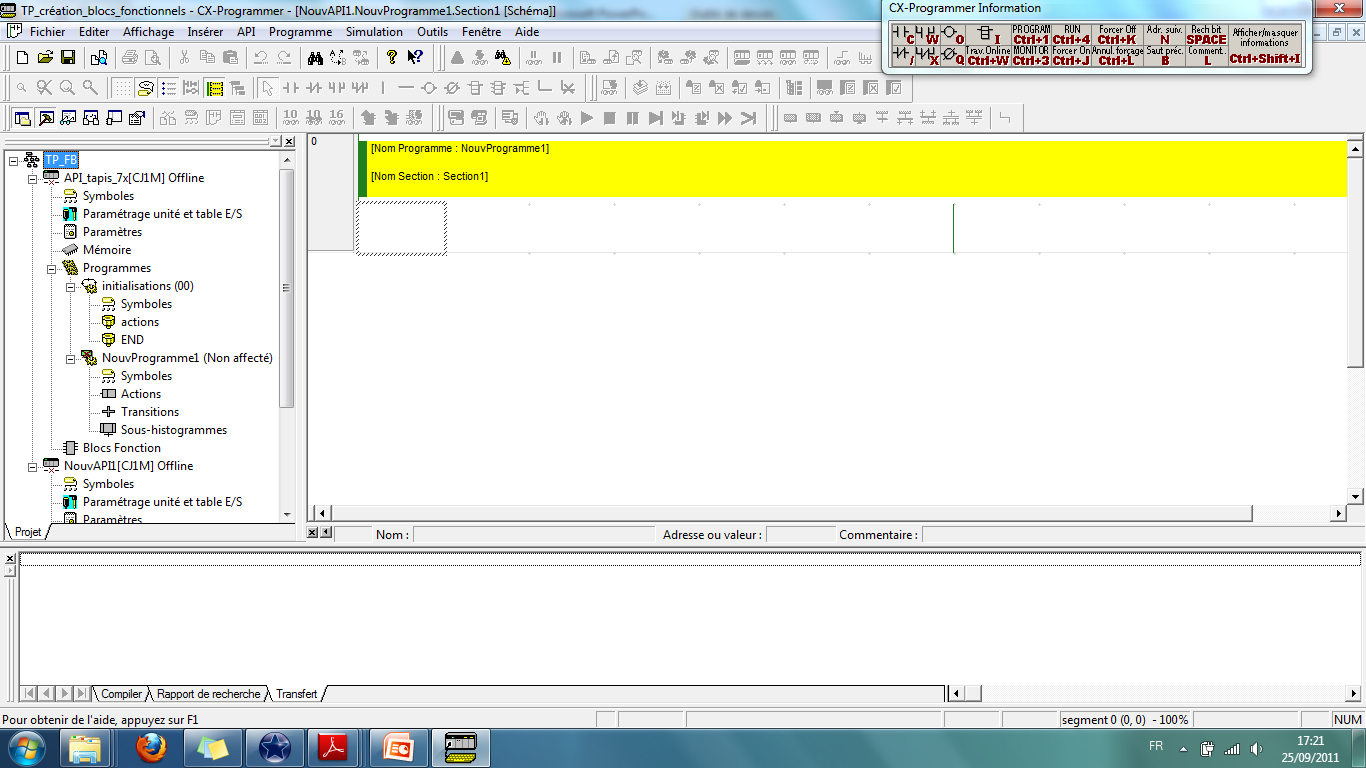
\includegraphics[trim = 50 510 1110 180, clip,height=6\fontcharht\font`\B]{images/unity_arbo}
			\end{minipage}
		\end{itemize}
	\item Les programmes (ou tâche)
	 	\begin{itemize}
		\item tous les programmes d'un automate sont exécutés \textbf{simultanément}
		\item chaque progamme peut avoir des variables locales (symboles)
		\item ils peuvent être écrits en SFC, FBD, LD, ST ou IL.
		\end{itemize}
\end{itemize}
\subsection{Les variables}
Les variables fournissent un moyen d'identifier des objets de données dont le contenu peut varier comme, par exemple, les données associées aux entrées/sorties.

\UPSTIaRetenir{\begin{itemize}
	Les variables sont un moyen de stoquer une donnée (le nombre de pièces dans un bac par exemple) ou de connaître l'état d'un capteur (par exemple la présence d'une pièce devant un capteur ou encore la température)
	\item Les variables (symboles) \textbf{globales} sont utilisables par toutes les tâches
	\item Les variables (symboles) \textbf{locales} à une tâche ne sont utilisables que par cette tâche.
\end{itemize}}

\UPSTIremarque{Dans \textit{Unity Pro}, les variables sont appelées 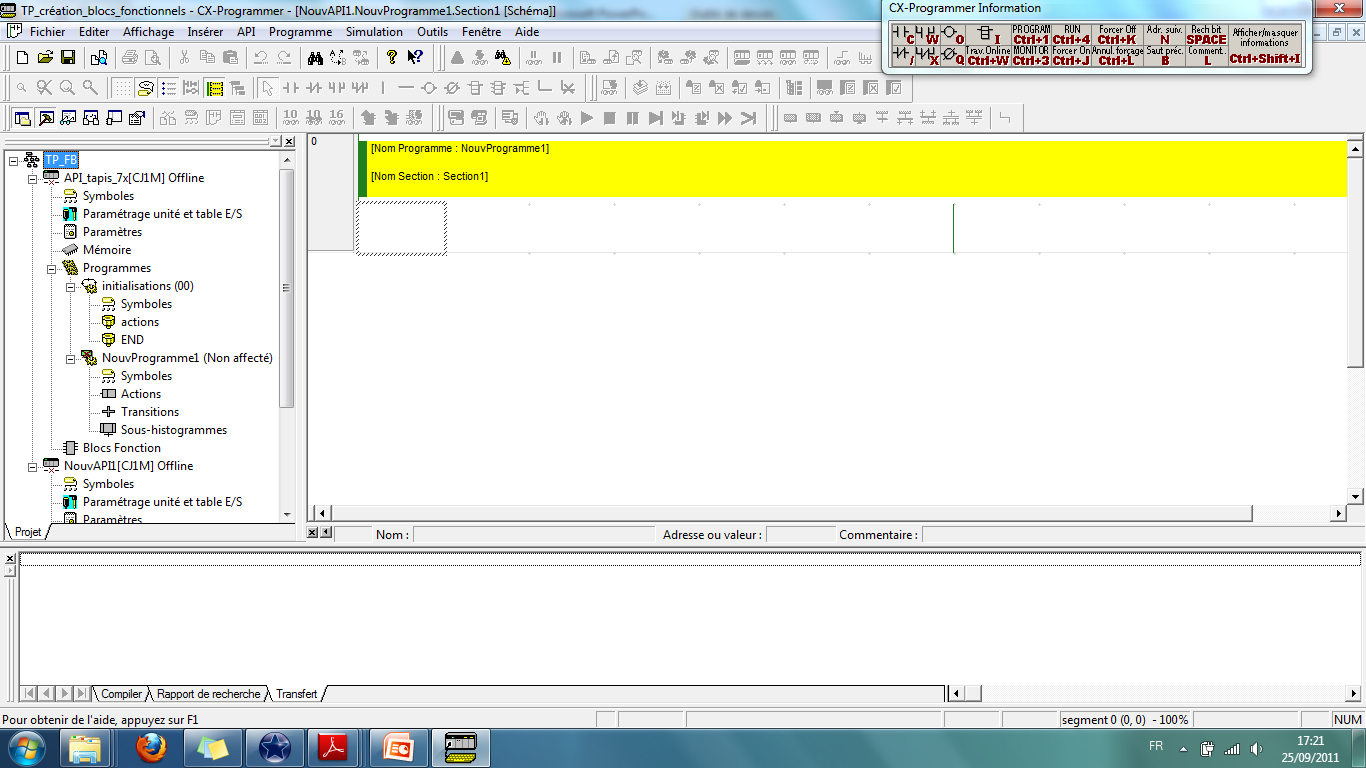
\includegraphics[trim = 100 457.5 1190 298, clip,height=\fontcharht\font`\B]{images/unity_arbo}, on trouve les variables \textbf{globales} dans les ressources de chaque API et les variables locales à chaque programme dans sa propre arborescence.}

Les variables sont donc stoquées dans la mémoire de l'automate. La mémoire d'un automate peut être vue comme une armoire gigantesques composée de différents "tiroirs" dans lesquelles on pourra stoquer une valeur. On représente souvent la mémoire par un tableau dans lequel on stoque une valeur par case. Une variable est donc stoquée dans une des cases du tableau. Le \textit{numéro} de la case est appelé \textbf{adresse} de la variable.

\UPSTIaRetenir[Adresse d'une variable]{
L'\textbf{adresse} d'une variable correspond à l'endroit où cette variable est stoquée dans la mémoire de l'automate.
}

Dans un automate, en plus des variables internes servant à stoquer des infomations, il faut pouvoir accéder aux différentes \textbf{entrées/sorties} de l'automate. Ces entrées/sorties sont également associées à des adresses.

Ces adresses sont d'une forme bien précise : \textbf{\%}\textbf{\color{green}Attribut}\textbf{\color{red}Type}\textbf{\color{blue}k.i.j}. Par exemple : \textbf{\%}\textbf{\color{green} Q}\textbf{\color{red}X}\textbf{\color{blue}2.4.F}.

\begin{table}[hb]
\centering
	\begin{tabular}{l|l|l}
\textbf{\color{green}Attribut}  & \textbf{\color{red}Type} & \textbf{\color{blue}k.j.i}\\%
%
\textbf{I} : Entrée             & \textbf{X} : Booléen      &  \textbf{k} : numéro de voie\\%
\textbf{Q} : Sortie             & \textbf{B} : 8 bits       &  \textbf{j} : numéro de carte\\%
\textbf{M} : Mémoire            & \textbf{W} : 16 bits      &  \textbf{i} : numéro de rack\\%
\textbf{K} : Constante          & \textbf{D} : 32 bits      &  \\%
                               & \textbf{F} : Flottant     &  \\%
\end{tabular} 

	\caption{décomposition d'une adresses}
\end{table}


\subsubsection{Différents types de variables}
En pratique, les variables que l'on stoque n'ont pas toutes le même type et ne nécessite pas la même taille de stockage.

\UPSTIexemple{On comprends aisément qu'un booléen (un seul bit qui ne peut valoir que \textbf{1} ou \textbf{0}) prend moins de place qu'un entier codé sur 8 bits pouvant prendre $2^8$ valeurs.}

Le Tableau~\ref{tab:types_de_donnees} représente les noms et types de données utilisés par les automates.
\begin{table}[h]
	\begin{tabular}{llcc}
\textbf{Nom} & \textbf{Type de données} & \textbf{Taille (bits)} & \textbf{Plage de valeurs}\\\hline
Boolean        & \textbf{BOOL}   & 1   &  0 (faux) ou 1 (vrai) \\\hline\hline%
%
Short integer  & \textbf{SINT}   & 8   &  $[-128 ; 127]$ \\\hline
Integer        & \textbf{INT}    & 16  &  $[-32768 ; 32767]$ \\\hline
Double interger& \textbf{DINT}   & 32  &  $[-2 147 483 648 ; 2 147 483 647]$ \\\hline\hline%
%
Unsigned Short integer  & \textbf{USINT}   & 8   &  $[0 ; 255]$ \\\hline
Unsigned Integer        & \textbf{UINT}    & 16  &  $[0 ; 65535]$ \\\hline
Unsigned Double interger& \textbf{UDINT}   & 32  &  $[0 ; 4294967295]$ \\\hline\hline%
%
Real number  & \textbf{REAL}   &  32   & $[-2^128 ; 2^128]$  \\\hline\hline%
%
Bit string of length 8  & \textbf{BYTE}   &   8  &  $[00 ; FF]$ \\\hline
Bit string of length 16  & \textbf{WORD}   &   16  &  $[0000 ; FFFF]$ \\\hline
Bit string of length 32  & \textbf{DWORD}   &   32  &  $[0000 ; FFFFFFFF]$ \\\hline\hline%
%
Time & \textbf{TIME} & & 0.0s à 21 474 836.47s \\
\end{tabular}

	\caption{Nom et tailles des différents types de données}
	\label{tab:types_de_donnees}
\end{table}


\end{document}
